\chapter{Results}
\label{Chap:Results}

Our proposal for this thesis was to create an all day wrist motion activity monitor
that was small, cost effective and comfortable.
This device would also have to be able to record data for an entire day of activity,
decided as 16 hours.
The final device we have created can worn on the wrist like a wrist watch by using its strap.
Figure \ref{Fig:WristPhoto} shows a photograph of this arrangement when the device is worn around a wrist.
In this chapter we consider how we have compared against the requirements for the wrist activity monitor that we had set.
Users are expected to wear the device at the start of the day,
and press a button to start recording wrist motion movement data.
At the end of the day,
this device can be connected to a computer though a USB port and the data that has been logged can be transferred.
This data can then be analyzed or processed on the computer as needed.
We use WristView, a modified version of a software previously created by our group to visually display the data logged by our device. 
\begin{figure}
\begin{center}
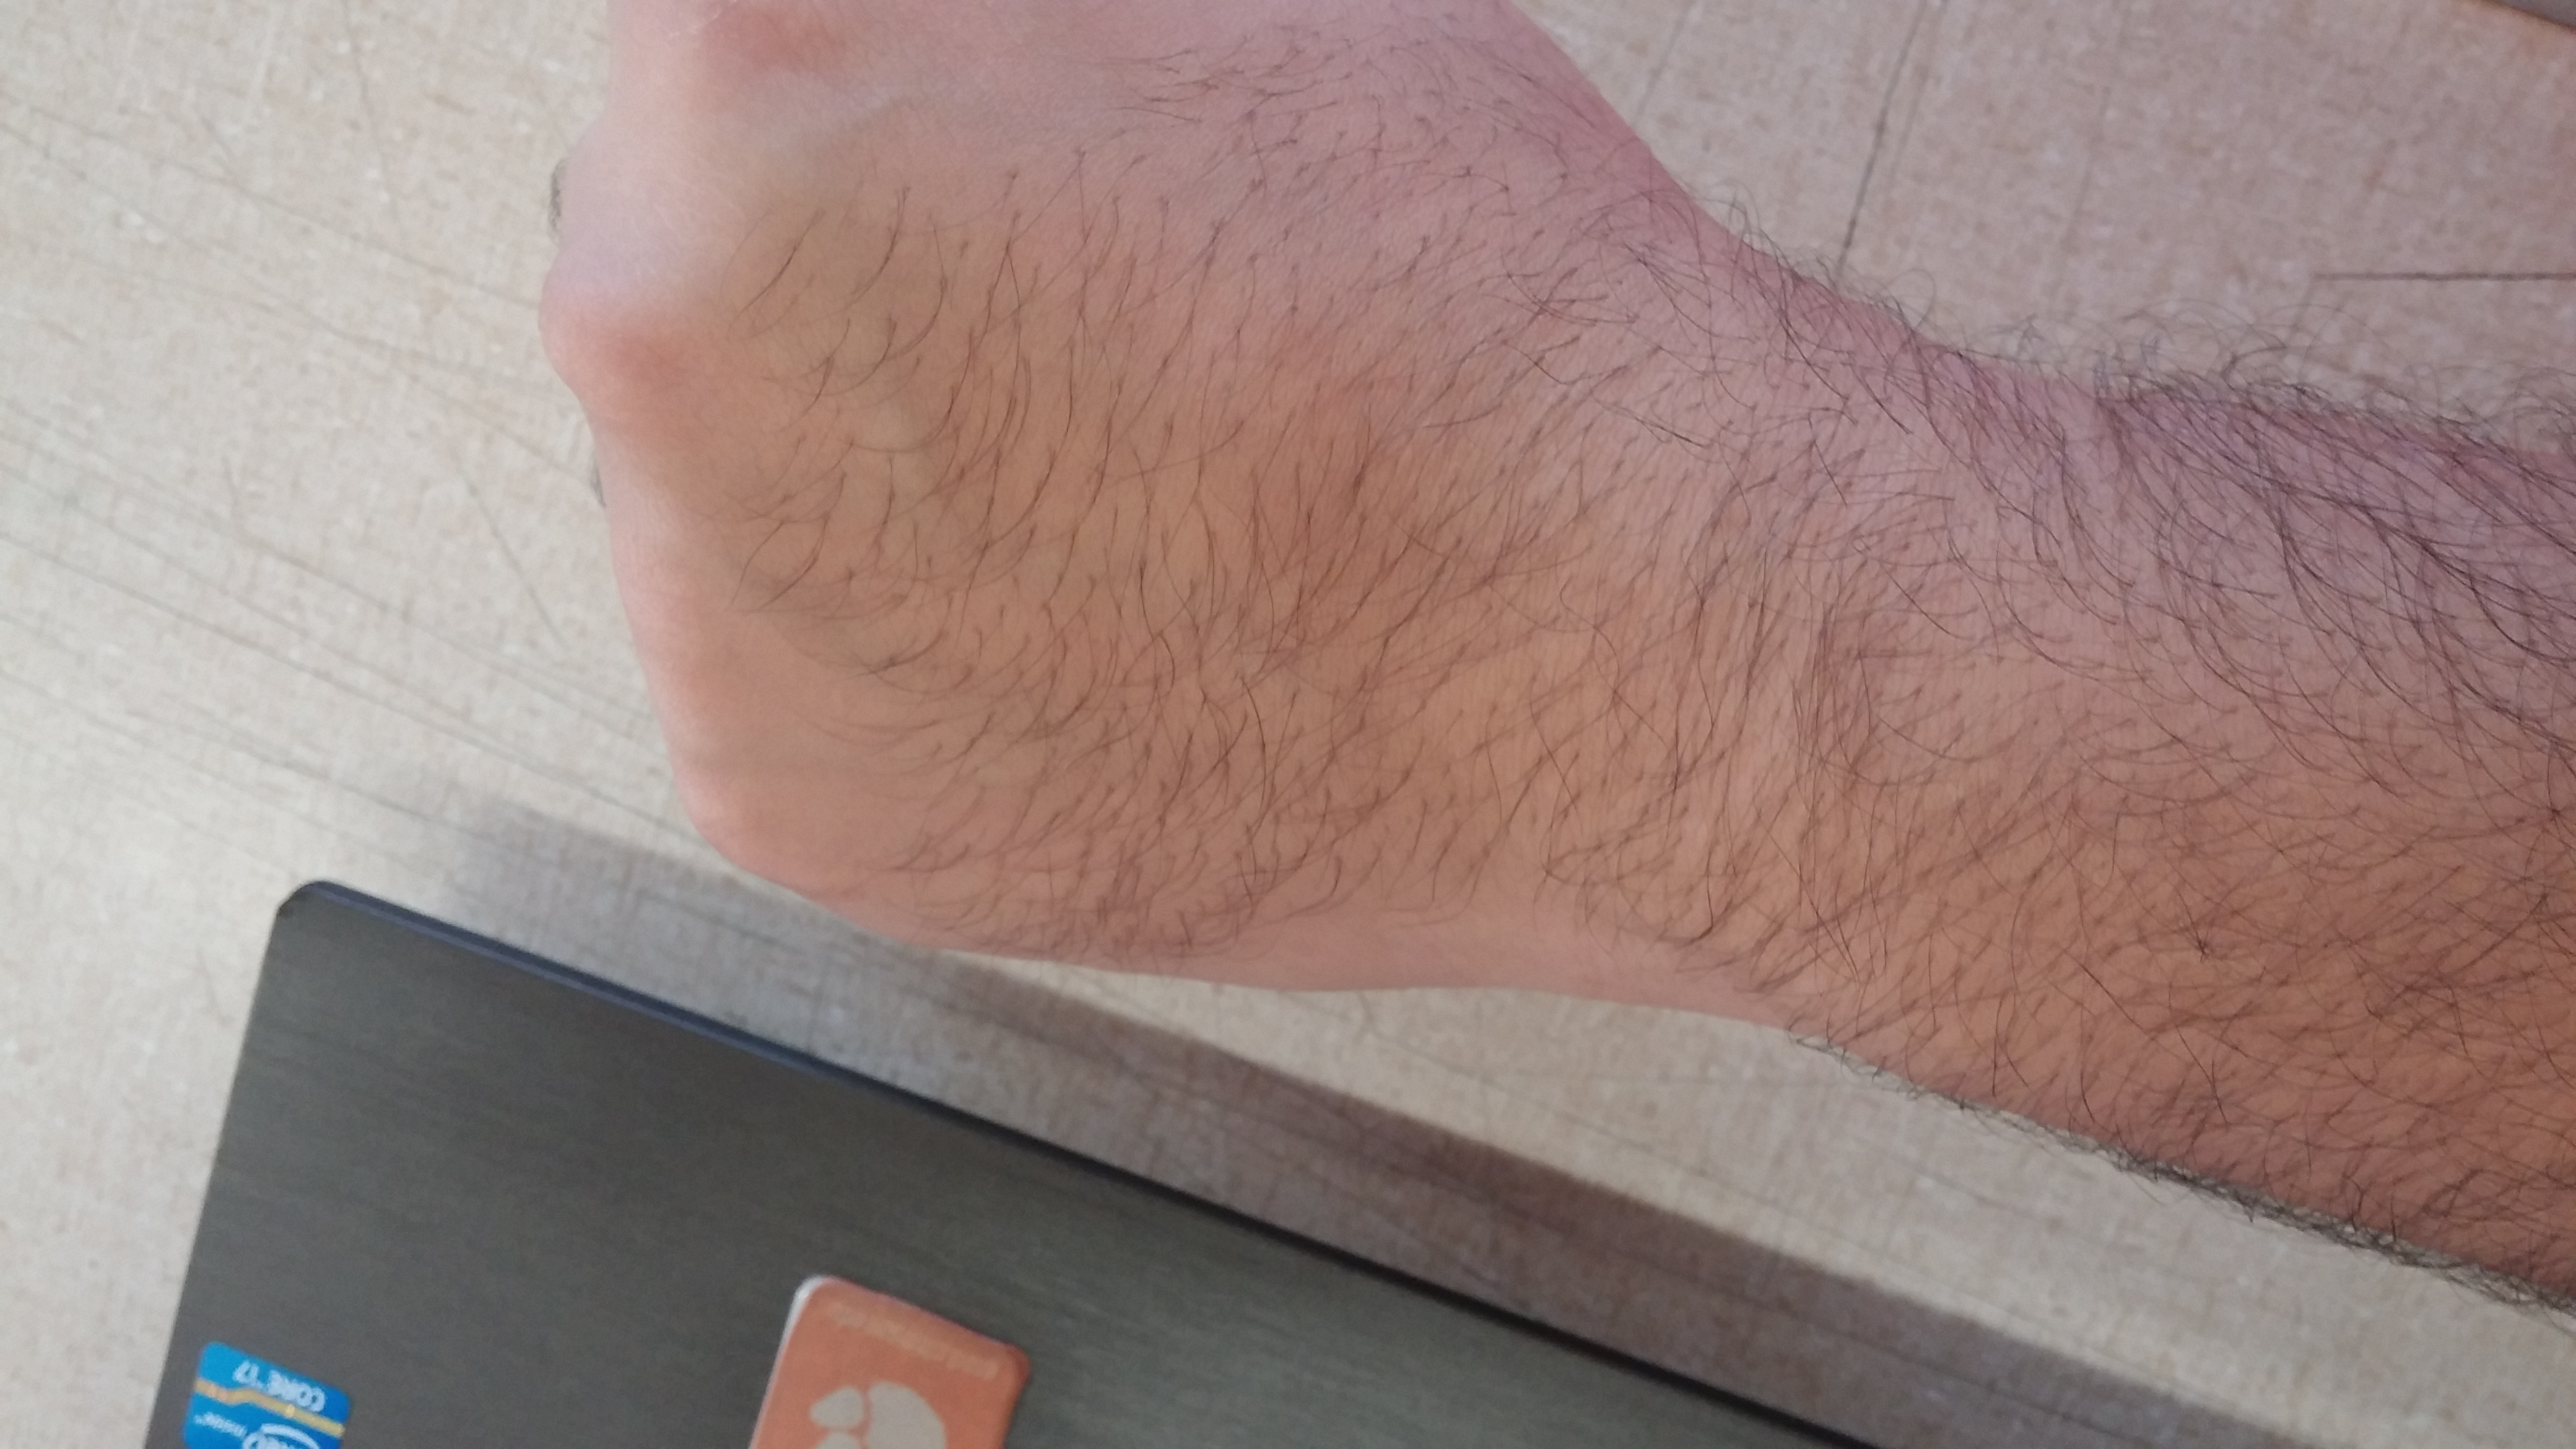
\includegraphics[width=\textwidth]{images/WristPhoto.jpg}
\caption{Photograph of the Activity Monitor mounted on a wrist.}
\label{Fig:WristPhoto}
\end{center}
\end{figure}

\section{Size and comfort}
\label{Sec:ResultsSize}
The final device fit comfortably inside OKW Enclosures' Ergo Minitec Small enclosure.
The dimensions of the device are the same as the enclosure,
52mm X 32mm X 15mm.
A strap that is 12cm wide and 20cm long allows the user to wear this device on their wrist.
The device weighs Xg, including the strap.
The device was tested by two volunteers for 10 hours each,
and reported to be similar to a wrist watch with regards to comfort.

\section{Battery Life}
\label{Sec:ResultsBatteryLife}
We would need to check if the battery life of the device meets our specifications.
Battery manufacturers are known to inflate the battery life on datasheets for their products.
Current draw and how the battery is used also changes the output capacity of the battery.
Section \ref{Sec:Programming} lays out the methods used to test our prototype,
and the techniques used to measure the battery life of the product.
After testing the battery three times,
we concluded that the 130mAh battery would log wrist motion data for at least 24 hours,
which was higher than the required battery life for our device,
16 hours.
On standyby mode (where the device is not recording any data), the battery life was up to one week.
Figure \ref{Fig:BatteryGraph} shows how the battery voltage drops versus time when it is actively recording motion data.
Data is not shown once the voltage dropped lower than 2.8V. The device was programmed to stop operating and enter standby mode once the voltage was lower then 2.8V. This was to avoid recording incorrect data or corrupting the memory chip once supply voltage was near the minimum level for devices on our circuit.

\begin{figure}
\begin{center}
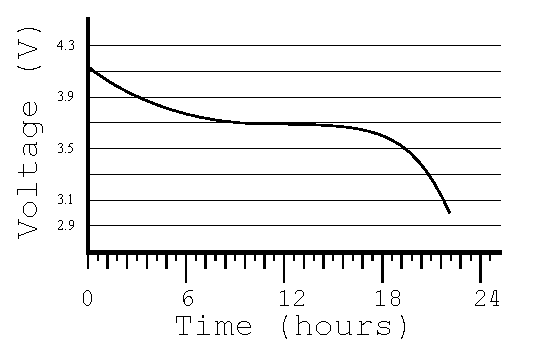
\includegraphics[width=0.7\textwidth]{images/BattLife.eps}
\caption{Graph showing Battery Life of the device.}
\label{Fig:BatteryGraph}
\end{center}
\end{figure}

\section{Software}
\label{Sec:ResultsSoftware}
We had been able to log data from the sensors into a memory chip,
and this data was then transferred to a computer in the form of a binary file.
Each bite in the file represents data recorded from a sensor,
with the time of the record being calculated by using the byte address.
Analysing this data as numbers is not something feasible for humans,
and we our much better at detecting patterns in visually displayed information.
Work done by our group previously could display motion data collected by an iPhone in a visual format.
We modified work done by Concha et al. \cite{concha2014study} and created our own software to display the data logged by the wrist motion activity tracker.
This software, as mentioned in section \ref{Sec:Software},
was named WristView and allowed us to visually compare data captured by the device.
A screenshot of WristView can be seen in figure \ref{Fig:WristView}.
The figure shows the data plotted as amplitude versus time.
For acceleration data the amplitude was in g's, where 1g = 9.8 m/s$^2$. For gyroscopes, the data was in deg/sec.
Raw data from sensors usually contains noise.
Also, the data isn't available at all times,
but instead in discrete time intervals, with 66ms between each point.
WristView can also smooth these signals based on code from PhoneView, which uses algorithm used by the research group previously \cite{concha2014study}. This can be seen in figure \ref{Fig:WristViewSoomth}
\begin{figure}
\begin{center}
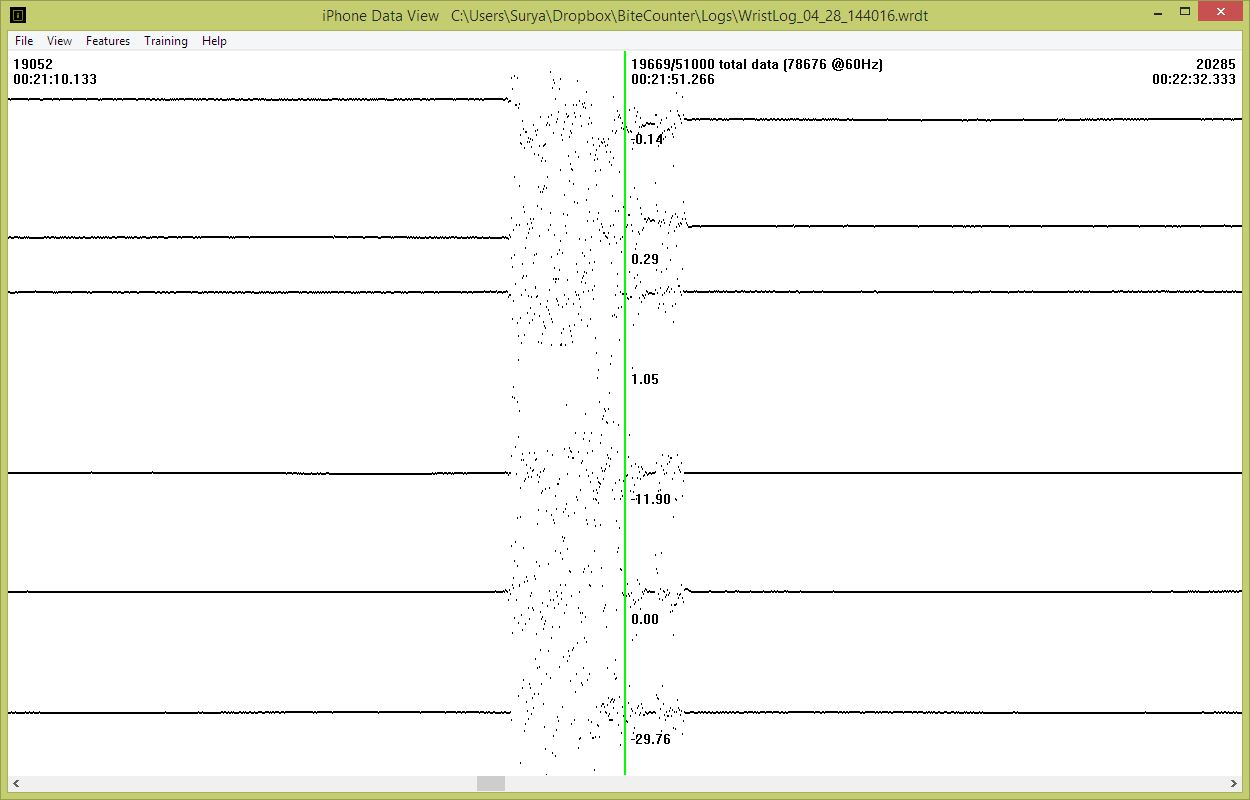
\includegraphics[width=0.7\textwidth]{images/WristView.jpg}
\caption{WristView displaying data captured by our prototype device. Top to bottom: Acceleration (X, Y, Z) and Angular Velocity (X, Y, Z)}
\label{Fig:WristView}
\end{center}
\end{figure}

\begin{figure}
\begin{center}
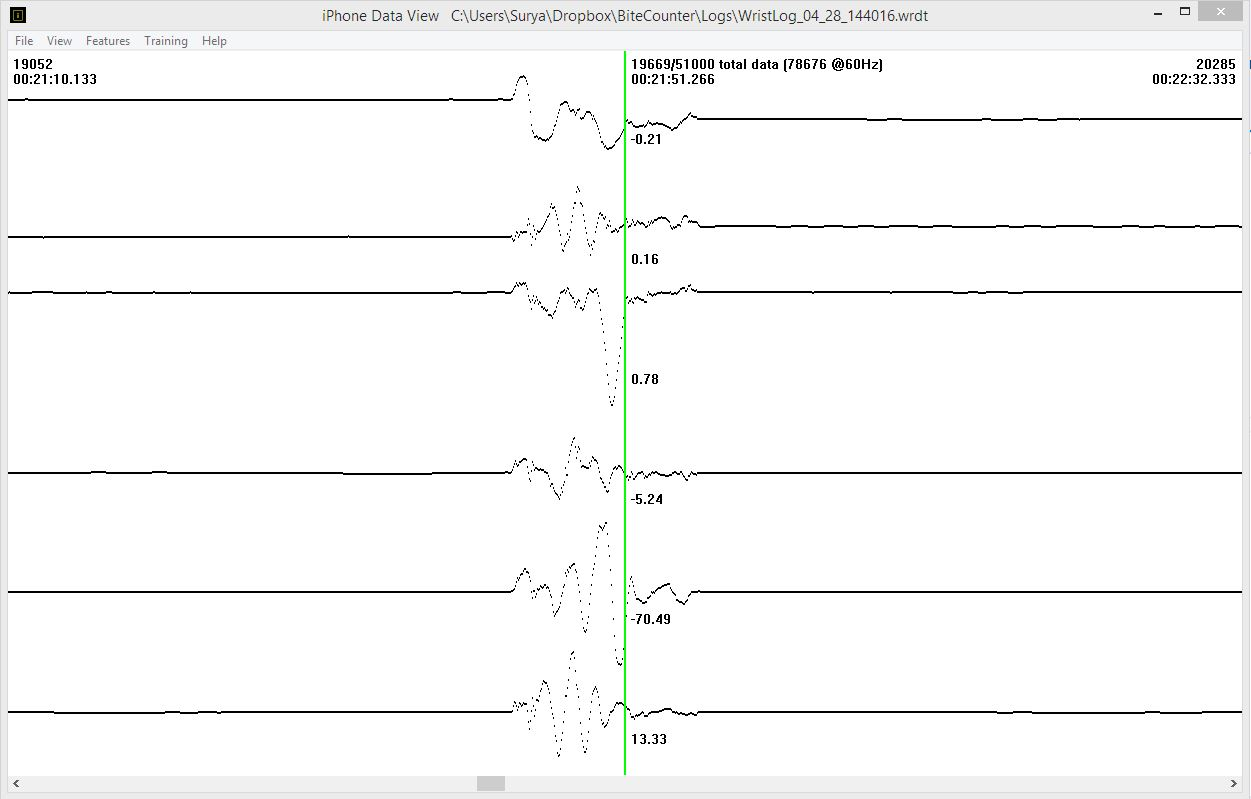
\includegraphics[width=0.7\textwidth]{images/WristSmooth.jpg}
\caption{WristView's smoothed data feature.}
\label{Fig:WristViewSoomth}
\end{center}
\end{figure}

\section{Device Cost}
\label{Sec:DevCost}
Earlier, we had mentioned the different devices on the market marketed as health monitors,
and also the high costs attached to using them.
The costs include expenditure on manufacturing and research.
After our device was created, 
we tabulated the cost of the parts of the device, and this can be seen in table \ref{BomTable}.
The total cost for the parts used per device was US\$52.5.
This number includes costs for PCB and stencil manufacture, but does not include any costs for the research of the device or hourly labour associated with writing code.
\inputfile{BOMTable.tex}


\section{Comparison of Devices}
\label{Sec:Comparison}
Activity Trackers like the Fitbit and Nike Fuelband created a new market segment of
wrist watch style activity trackers.
Other improvments in technology have allowed multiple manufacturers to launch new
wrist based smart watches in the past two years,
with a major rush in the past two months.
Another market segement uses wrist motion or gestures to control computers / digital devices.
These devices may be able to support the different bite counting and meal detection algorithsm created by our group.
We compared our wrist motion activity tracker to the different wrist mounted devices on the market
including some new ones that have been announced but are yet to release in the United States of America.
Table \ref{Tab:DevCompare} select devices and their important parameters.
Our requirements call for a device that can record data from an accelerometer and gyroscope for 24 hours,
and be comfortable to wear for that period repeatedly. Comparison in Table \ref{Tab:DevCompare} shows that our device performs better than other devices on the market for our specific purpose, and that most devices lack the support for our bite counting application while maintaining comfort.
\inputfile{CompTable.tex}
\chapter{Conclusion and Future Work}
\label{Chap:Concl}
In this thesis, we proposed to create a device that would record information on 
the movement of a human wrist during a day.
This was motivated by the fact that wrist motion information can be used to count the number of bites
taken by a user,
or predict the tool being used to take a bite.
The device could be worn for extended intervals of time
without causing discomfort to the user.
As mentioned in Results (Chapter \ref{Chap:Results}),
we were able to create a wrist motion activity tracker that records data at good resolution
for our purpose of detecting periods of eating or non-eating, 
or for our purpose of counting the number of bites taken.
At this point of time,
the device has a button that allows the device to be turned on and off.
When the device is turned off,
it enters standby mode,
and returns to recording data when turned on again.
This data is recorded serially,
and the device has no concept of local time.

In the future,
we aim to solve this problem by adding a time synchronization feature when the device is connected to a computer.
This would store the local time of the user on the wrist motion activity tracker,
and will allow the device to time stamp when it was stopped and started,
allowing data analysis to be performed to detect periods of eating and non-eating.

In our wrist motion activity tracker,
a large amount of power is utilized by the sensors which are always turned on.
While we were working through this thesis,
newer technology has allowed sensor manufacturers to improve the sensors they are producing.
Some new sensors now come with microcontrollers in-built which can be programmed by the user.
In our thesis,
the sensors we used
were operating based on an internal clock of 8Hz.
We would then read from the sensors at 15Hz.
Since we only need the sensors to be polled at 15Hz,
it should be possible to decrease the rate at which the sensors are operating.
If the sensors could sleep between two pools,
it would allow us to have a huge improvement in battery life as it would reduce the average current draw by the sensors.

When we compared the different devices on the market,
we noticed that the wrist band device MYO uses EMG sensors coupled with accerlerometer and gyroscope data to increase the accuracy of detection.
Thalmic Labs \cite{Web:GetMyo} claims that the EMG sensors help pin point the pose of a users hand.
We consider that this claim might be true,
based on newer EMG sensors that are smaller and comfortable to wear around the wrist,
we plan to incorporate these sensors in future work.